\documentclass[a4paper]{article}

\usepackage{inputenc}
\usepackage[british,UKenglish]{babel}
\usepackage{amsmath}
%\usepackage{titlesec}
\usepackage{color}
\usepackage{graphicx}
\usepackage{fancyref}
\usepackage{hyperref}
\usepackage{float}
\usepackage{scrextend}
\usepackage{setspace}
\usepackage{xargs}
\usepackage{multicol}
\usepackage{nameref}

\usepackage{sectsty}
\usepackage{multicol}
\usepackage{multirow}
\usepackage[procnames]{listings}
\usepackage{appendix}

\newcommand\tab[1][1cm]{\hspace*{#1}}
\hypersetup{colorlinks=true, linkcolor=black}
\interfootnotelinepenalty=10000

\newcommand{\cleancode}[1]{\begin{addmargin}[3em]{3em}\texttt{\textcolor{cleanOrange}{#1}}\end{addmargin}}
\newcommand{\cleanstyle}[1]{\text{\textcolor{cleanOrange}{\texttt{#1}}}}


\usepackage[colorinlistoftodos,prependcaption,textsize=footnotesize]{todonotes}
\newcommandx{\commred}[2][1=]{\textcolor{Red}
{\todo[linecolor=red,backgroundcolor=red!25,bordercolor=red,#1]{#2}}}
\newcommandx{\commblue}[2][1=]{\textcolor{Blue}
{\todo[linecolor=blue,backgroundcolor=blue!25,bordercolor=blue,#1]{#2}}}
\newcommandx{\commgreen}[2][1=]{\textcolor{OliveGreen}{\todo[linecolor=OliveGreen,backgroundcolor=OliveGreen!25,bordercolor=OliveGreen,#1]{#2}}}
\newcommandx{\commpurp}[2][1=]{\textcolor{Plum}{\todo[linecolor=Plum,backgroundcolor=Plum!25,bordercolor=Plum,#1]{#2}}}

\def\code#1{{\tt #1}}

\def\note#1{\noindent{\bf [Note: #1]}}

\makeatletter
%% The "\@seccntformat" command is an auxiliary command
%% (see pp. 26f. of 'The LaTeX Companion,' 2nd. ed.)
\def\@seccntformat#1{\@ifundefined{#1@cntformat}%
   {\csname the#1\endcsname\quad}  % default
   {\csname #1@cntformat\endcsname}% enable individual control
}
\let\oldappendix\appendix %% save current definition of \appendix
\renewcommand\appendix{%
    \oldappendix
    \newcommand{\section@cntformat}{\appendixname~\thesection\quad}
}
\makeatother


% "define" Scala
\usepackage[T1]{fontenc}  
\usepackage[scaled=0.82]{beramono}  
\usepackage{microtype} 

\sbox0{\small\ttfamily A}
\edef\mybasewidth{\the\wd0 }

\lstdefinelanguage{scala}{
  morekeywords={abstract,case,catch,class,def,%
    do,else,extends,false,final,finally,%
    for,if,implicit,import,match,mixin,%
    new,null,object,override,package,%
    private,protected,requires,return,sealed,%
    super,this,throw,trait,true,try,%
    type,val,var,while,with,yield},
  sensitive=true,
  morecomment=[l]{//},
  morecomment=[n]{/*}{*/},
  morestring=[b]",
  morestring=[b]',
  morestring=[b]"""
}

\usepackage{color}
\definecolor{dkgreen}{rgb}{0,0.6,0}
\definecolor{gray}{rgb}{0.5,0.5,0.5}
\definecolor{mauve}{rgb}{0.58,0,0.82}

% Default settings for code listings
\lstset{frame=tb,
  language=scala,
  aboveskip=3mm,
  belowskip=3mm,
  showstringspaces=false,
  columns=fixed, % basewidth=\mybasewidth,
  basicstyle={\small\ttfamily},
  numbers=none,
  numberstyle=\footnotesize\color{gray},
  % identifierstyle=\color{red},
  keywordstyle=\color{blue},
  commentstyle=\color{dkgreen},
  stringstyle=\color{mauve},
  frame=single,
  breaklines=true,
  breakatwhitespace=true,
  procnamekeys={def, val, var, class, trait, object, extends},
  procnamestyle=\ttfamily\color{red},
  tabsize=2
}

\lstnewenvironment{scala}[1][]
{\lstset{language=scala,#1}}
{}
\lstnewenvironment{cpp}[1][]
{\lstset{language=C++,#1}}
{}
\lstnewenvironment{bash}[1][]
{\lstset{language=bash,#1}}
{}
\lstnewenvironment{verilog}[1][]
{\lstset{language=verilog,#1}}
{}



%代码段设置
\lstset{numbers=left,
basicstyle=\tiny,
numberstyle=\tiny,
keywordstyle=\color{blue!70},
commentstyle=\color{red!50!green!50!blue!50},
frame=single, rulesepcolor=\color{red!20!green!20!blue!20},
escapeinside=``
}

\graphicspath{ {images/} }
\usepackage{ctex}
\usepackage{graphicx}
\usepackage{color,framed}%文本框
\usepackage{listings}
\usepackage{caption}
\usepackage{amssymb}
\usepackage{enumerate}
\usepackage{xcolor}
\usepackage{bm} 
\usepackage{lastpage}%获得总页数
\usepackage{fancyhdr}
\usepackage{tabularx}  
\usepackage{geometry}
\usepackage{minted}
\usepackage{graphics}
\usepackage{subfigure}
\usepackage{float}
\usepackage{pdfpages}
\usepackage{pgfplots}
\pgfplotsset{width=10cm,compat=1.9}
\usepackage{multirow}
\usepackage{footnote}
\usepackage{booktabs}
\usepackage{url}

%-----------------------伪代码------------------
\usepackage{algorithm}  
\usepackage{algorithmicx}  
\usepackage{algpseudocode}  
\floatname{algorithm}{Algorithm}  
\renewcommand{\algorithmicrequire}{\textbf{Input:}}  
\renewcommand{\algorithmicensure}{\textbf{Output:}} 
\usepackage{lipsum}  
\makeatletter
\newenvironment{breakablealgorithm}
  {% \begin{breakablealgorithm}
  \begin{center}
     \refstepcounter{algorithm}% New algorithm
     \hrule height.8pt depth0pt \kern2pt% \@fs@pre for \@fs@ruled
     \renewcommand{\caption}[2][\relax]{% Make a new \caption
      {\raggedright\textbf{\ALG@name~\thealgorithm} ##2\par}%
      \ifx\relax##1\relax % #1 is \relax
         \addcontentsline{loa}{algorithm}{\protect\numberline{\thealgorithm}##2}%
      \else % #1 is not \relax
         \addcontentsline{loa}{algorithm}{\protect\numberline{\thealgorithm}##1}%
      \fi
      \kern2pt\hrule\kern2pt
     }
  }{% \end{breakablealgorithm}
     \kern2pt\hrule\relax% \@fs@post for \@fs@ruled
  \end{center}
  }
\makeatother
%------------------------代码-------------------
\usepackage{xcolor} 
\usepackage{listings} 
\lstset{ 
breaklines,%自动换行
basicstyle=\small,
escapeinside=``,
keywordstyle=\color{ blue!70} \bfseries,
commentstyle=\color{red!50!green!50!blue!50},% 
stringstyle=\ttfamily,% 
extendedchars=false,% 
linewidth=\textwidth,% 
numbers=left,% 
numberstyle=\tiny \color{blue!50},% 
frame=trbl% 
rulesepcolor= \color{ red!20!green!20!blue!20} 
}

%-------------------------页面边距--------------
\geometry{a4paper,left=2.3cm,right=2.3cm,top=2.7cm,bottom=2.7cm}
%-------------------------页眉页脚--------------
\usepackage{fancyhdr}
\pagestyle{fancy}
\lhead{\kaishu \leftmark}
% \chead{}
\rhead{\kaishu 并行程序设计实验报告}%加粗\bfseries 
\lfoot{}
\cfoot{\thepage}
\rfoot{}
\renewcommand{\headrulewidth}{0.1pt}  
\renewcommand{\footrulewidth}{0pt}%去掉横线
\newcommand{\HRule}{\rule{\linewidth}{0.5mm}}%标题横线
\newcommand{\HRulegrossa}{\rule{\linewidth}{1.2mm}}
\setlength{\textfloatsep}{10mm}%设置图片的前后间距
%--------------------文档内容--------------------

\begin{document}
\renewcommand{\contentsname}{目\ 录}
\renewcommand{\appendixname}{附录}
\renewcommand{\appendixpagename}{附录}
\renewcommand{\refname}{参考文献} 
\renewcommand{\figurename}{图}
\renewcommand{\tablename}{表}
\renewcommand{\today}{\number\year 年 \number\month 月 \number\day 日}

%-------------------------封面----------------
\begin{titlepage}
    \begin{center}
    
\includegraphics[width=0.8\textwidth]{NKU.png}\\[1cm]
    \vspace{20mm}
		\textbf{\huge\textbf{\kaishu{计算机学院}}}\\[0.5cm]
		\textbf{\huge{\kaishu{并行程序设计期末报告}}}\\[2.3cm]
		\textbf{\Huge\textbf{\kaishu{联想Y7000P 2021 体系结构调研}}}

		\vspace{\fill}
    
    % \textbf{\Large \textbf{并行程序设计期末实验报告}}\\[0.8cm]
    % \HRule \\[0.9cm]
    % \HRule \\[2.0cm]
    \centering
    \textsc{\LARGE \kaishu{姓名\ :\ 卢麒萱}}\\[0.5cm]
    \textsc{\LARGE \kaishu{学号\ :\ 2010519}}\\[0.5cm]
    \textsc{\LARGE \kaishu{专业\ :\ 计算机科学与技术}}\\[0.5cm]
    
    \vfill
    {\Large \today}
    \end{center}
\end{titlepage}

\renewcommand {\thefigure}{\thesection{}.\arabic{figure}}%图片按章标号
\renewcommand{\figurename}{图}
\renewcommand{\contentsname}{目录}  
\cfoot{\thepage\ of \pageref{LastPage}}%当前页 of 总页数


% 生成目录
\clearpage
\tableofcontents
\newpage

%--------------------------Title--------------------------------
\section{引言}
\subsection{国内外并行硬件体系结构发展现状}
并行计算机对于国家安全等重要领域有着举着轻重的作用。我国的并行计算研究始终紧跟国际步伐,尽管在方面开展的研究和应用较早,也拥有很多的并行计算资源,但成效相对美日等发达国家还存在较大的差距,在研究中形成了“理论-设计-实现-应用”的一体化并行计算研究体系。但并行计算的发展依旧是参差不齐的,目前并行应用的效率依然较低,无法高效的使用并行计算机的资源,导致大量资源闲置。并行程序编写难度较大,并行编程语言对于一般的编程人员还不够简单易行,也缺乏高效的并行编程环境工具, 并行计算机本身的构建也存在着能耗过大、管理困难、可扩展性差等方面的问题。

当前,并行机发展基本状况可以大致归纳为:
\begin{itemize}
  \item 并行软件的发展远远落后于并行计算体系结构的发展;
  \item 并行计算的应用远远落后于并行计算技术的发展;
  \item 大规模并行处理系统已不再是主要研究领域;
  \item 有高速网联成的各种类型、规模可伸缩计算机群,将进一步促使并行计算应用的发展;
  \item 计算系统的可扩展和可编程性已成为并行机未来发展的一对主要矛盾.
\end{itemize}

并行性包括时间并行性和空间并行性两部分。一般时间并行性的开发采用资源共享和时间重叠的方法,而空间并行性的提高则采用资源重复的方法。大规模并行结构尚有三大难题:节点负载均衡问题,Cache一致性问题和通讯同步问题,均为全局优化问题。冯・诺依曼结构的一维顺序存储模型严重地制约了并行体系结构的发展,在此基础上进行并行性的挖掘只能有限地提高计算机性能。
\subsection{国内外并行硬件体系结构发展趋势}
在并行机硬件与用户需求之间有一巨大间隔,只能靠软件来填补。并行计算机的应用效率和可用性主要取决于并行软件。计算能力并不是衡量超级计算机的唯一重要标准,拿天河二号为例,它的运算能力世界第一,但是功能却远远落后于美国等国家的超级计算机。并行算法的效率与体系结构密切相关。将常用的并行算法经充分优化后做成并行算法库供用户调用, 将目前广泛使用的库函数并行化变成标准的并行库函数, 这是推广并行机必须要做的事, 也是提高并行机实际性能的关键技术。 

多核技术的出现与主流化, 对于并行计算体系结构、并行算法、并行程序设计与并行应用的研究都分别产生了重要的影响,带来了新的挑战。一般说来,超级计算机系统可分为两大部分,一部分是包括硬件和系统软件的平台,另一部分是应用软件。对不具有可编程性的超级计算机,即使平台有较高的性价比,但却大大增加了移植原有应用软件的难度和开发新的应用软件的成本,从而导致整个系统的性价比大幅度下降。多核化趋势正在改变并行计算的面貌,人们开始不再仅仅关注并行计算机的高性能,也开始关注高效能。多核技术对并行计算机系统的算法和编程带来了很大的困难,程序代码迁移也是个问题,需要有一个清晰的迁移策略,来使其代码可以最大化地利用多核硬件资源,同时为之付出的迁移代价要尽可能的小。未来的并行计算机系统需要去适应多核系统的发展,多核技术促进了并行编程的普及以及并行程序设计的进步,降低了物理上共享存储的并行处理平台的门槛。

\subsection{选题目的及意义}
联想拯救者系列,是当前国内市面上中高端定位主流游戏本系列。而Y7000P 2021款,也是畅销一时的大热机型,在同价位机型中性价比突出,深受民众青睐。本文意通过对该并行计算机体系结构进行调研与剖析,了解当前主流家用并行计算机架构的发展现状,同时与最新产品作对比,印证并行计算机未来的发展所趋。

%-------------------------Codes----------------------------------
\section{体系结构}
\subsection{参数概览}
\begin{table}[!htbp]
\centering
\begin{tabular}{|c|c|}
\hline
处理器&Intel Core i7-11800H(2.3GHz/L3 24M)\\
\hline
核心/线程& 八核心/十六线程\\
\hline
总线规格& DMI3 8GT/s\\
\hline
核心架构& Tiger Lake-H\\
\hline
处理器系列& 第11代酷睿i7\\
\hline
处理器主频& 2.3GHz\\
\hline
最高频率& 4.6GHz\\
\hline
三级缓存& L3 24M\\
\hline
制程工艺& 10nm\\
\hline
功耗& 80W(高耗电)\\
\hline
\end{tabular}
\caption{处理器}
\end{table}

\begin{table}[!htbp]
\centering
\begin{tabular}{|c|c|}
\hline
显卡类型& 独立显卡\\
\hline
显卡芯片& NVIDIA Geforce RTX 3060\\
\hline
显存容量& 6GB\\
\hline
显存位宽& 192bit\\
\hline
显存类型& GDDR6\\
\hline
显卡性能& 支持光线追踪,支持DirectX 12\\
\hline
\end{tabular}
\caption{显示卡}
\end{table}

\subsection{CPU}
酷睿i7-11800H作为英特尔的主流产品,用于大多数中高端笔记本电脑。搭载着英特尔推出的笔记本处理器11代酷睿,代号Tiger Lake,使用10nm+工艺,集成全新的Willow Cove CPU架构、Xe架构的Gen12 GPU核显,并大大地强化了AI能力,最高加速频率可达5GHz。11800H配备8个核心和16个线程,24MB的L3缓存,2.3GHz的基本频率,功耗为45W,睿频加速2个核心可达4.6GHz,全核可达4.2GHz。Xe集成GPU有32个执行单元,频率速度高达1450 MHz。
\subsubsection{Tiger Lake}
Tiger Lake是英特尔第 11 代英特尔酷睿移动处理器的代号,它基于全新的Willow Cove Core微架构,采用英特尔第三代10 纳米工艺节点 10SF(“10 纳米 SuperFin”)制造。Tiger Lake 取代了Ice Lake系列移动处理器,代表了英特尔流程-架构-优化模型中的优化步骤。

\begin{table}[!htbp]
\centering
\begin{tabular}{|c|c|}
\hline
技术节点& 英特尔 10 纳米 SuperFin (10SF) 工艺\\
\hline
架构& 	x86-64\\
\hline
微架构& 	Willow Cove\\
\hline
指令& x86-64\\
\hline
核心& 2–8\\
\hline
GPU& 	基于 Intel Xe的集成显卡\\
\hline
\end{tabular}
\caption{Tiger Lake架构和规格}
\end{table}

核心是英特尔最新的 Willow Cove 处理器内核,具有 1.25 MB 的专有 L2 缓存和每个内核高达 3 MB 的共享 L3 缓存,以及英特尔最新的 Xe-LP 显卡。 这些都从 6 核和 12 线程开始,并为最昂贵的型号提供高达 5.0 GHz 的单核涡轮增压。

英特尔的顶级 Tiger Lake 'Core 11 th Gen' 处理器,即 Core i7-1185G7。这是具有超线程的四核处理器,总共提供八个线程。该处理器还具有全尺寸的新 X e -LP 图形,具有 96 个运行单元,运行频率高达 1450 MHz。
\begin{table}[!htbp]
\centering
\begin{tabular}{|c|c|}
\hline
核心线程& 4核8线程\\
\hline
12 W 时的基本频率& 	1200兆赫\\
\hline
15 W 时的基本频率& 	1800兆赫\\
\hline
28 W 时的基本频率& 3000兆赫\\
\hline
高达 50 W的1C Turbo & 4800兆赫\\
\hline
高达 50 W 的全核 Turbo& 4300兆赫\\
\hline
二级缓存& 每个核心 1.25 MB\\
\hline
三级缓存& 12 MB\\
\hline
集成显卡& Xe-LP
96 执行单元
1350 MHz Turbo\\
\hline
内存支持& 32 GB LPDDR4X-4266
或
64 GB DDR4-3200\\
\hline
\end{tabular}
\caption{Intel Core i7-1185G7 'Tiger Lake'}
\end{table}

在 12 W 时,英特尔列出了 1.2 GHz 的基本频率,而在 28 W 时,英特尔列出了 3.0 GHz 的基本频率。在 12 W 和 28 W 场景中,处理器可以在一个核心/两个线程上加速到 4.8 GHz。该系统专为散热或电源问题而设计,因此 CPU 在两种模式下均可提升至 4.8 GHz。不仅如此,对于任何 TDP 设置,在 Turbo 模式下的功耗都被限制为 55 W。
\subsubsection{i7-11800H测评}

根据ZMMOO的性能测评,有以下的测评结果图参考。


\begin{figure}[H] %H为当前位置,!htb为忽略美学标准,htbp为浮动图形
\centering %图片居中
\includegraphics[width=0.7\textwidth]{多} %插入图片,[]中设置图片大小,{}中是图片文件名
\caption{Cinebench R20多线程性能} %最终文档中希望显示的图片标题
\label{Fig.main2} %用于文内引用的标签
\end{figure}

多线程方面酷睿i7-11800H比酷睿i7-10870H快了35\%,比i7-10750H领先近60\%。

尽管比上一代有巨大的进步,但英特尔所能实现的性能只能和AMD上一代的Ryzen 7 4800H媲美;11800H仍然比5800H慢9\%。

\begin{figure}[H] %H为当前位置,!htb为忽略美学标准,htbp为浮动图形
\centering %图片居中
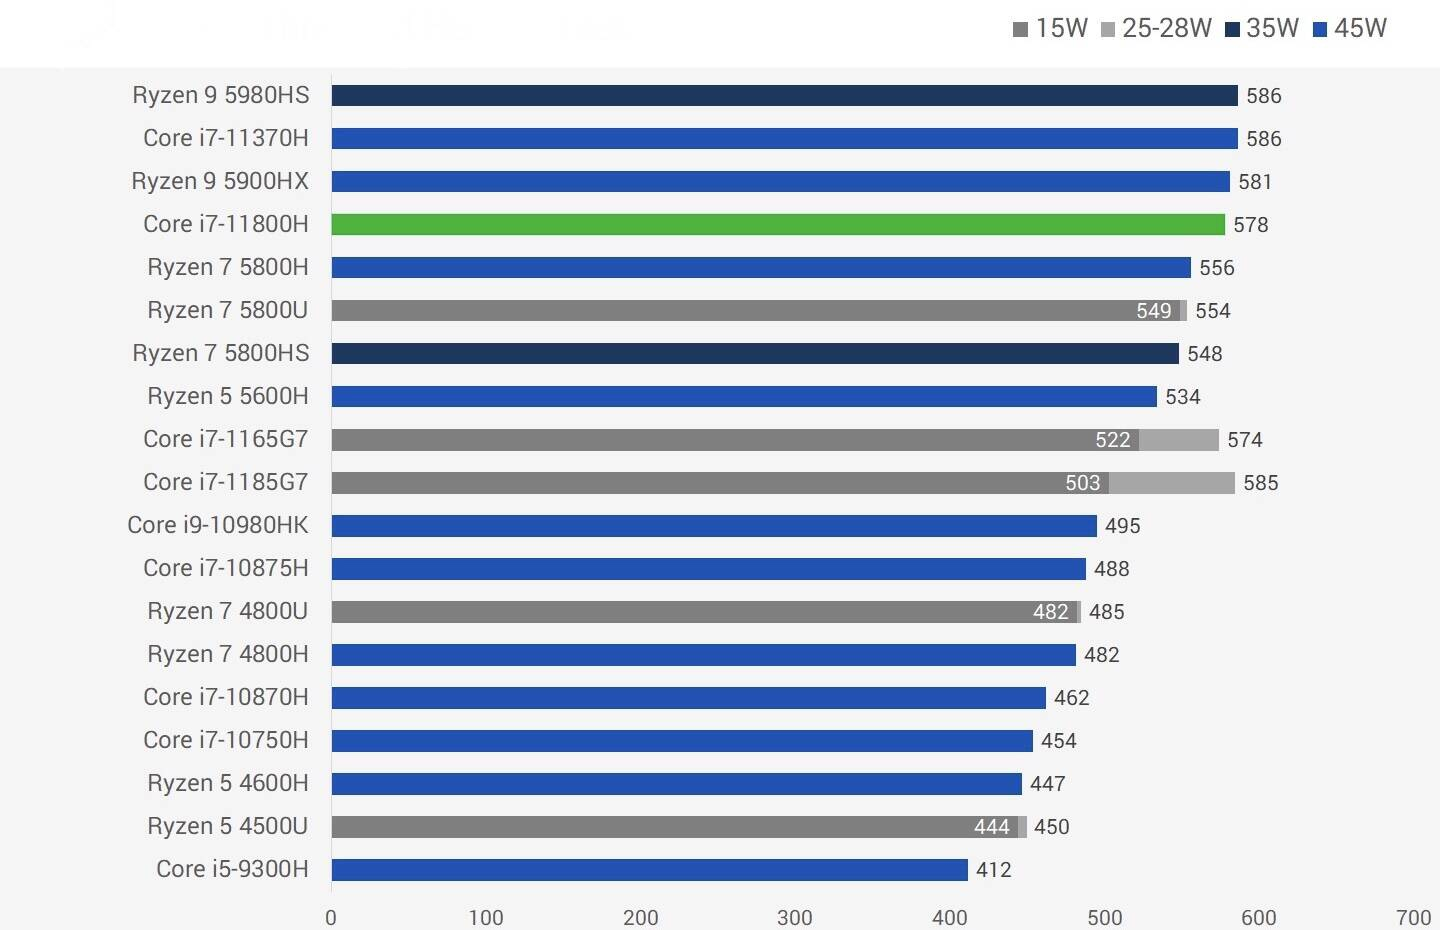
\includegraphics[width=0.7\textwidth]{单} %插入图片,[]中设置图片大小,{}中是图片文件名
\caption{Cinebench R20单线程性能} %最终文档中希望显示的图片标题
\label{Fig.main2} %用于文内引用的标签
\end{figure}

虽然英特尔在多线程方面无法与AMD匹敌,但正如表中所示,Tiger Lake的单线程性能很强。即使频率只有4.6GHz,11800H也比5800H高出4\%,这使它的性能与AMD更高级别的Ryzen 9 5900HX相近。5900HX的频率也达到了4.6GHz。

\subsubsection{12代与11代酷睿对比}

第12代英特尔®酷睿™产品家族包括60款处理器,为来自合作伙伴的500多种机型设计提供动力。根据2021年英特尔架构日介绍,首次采用Intel 7制程工艺的全新高性能混合架构,带来了从9瓦到125瓦的可扩展性能,为从超轻薄笔记本电脑到发烧友台式机的每一个PC细分市场以及边缘计算设备提供卓越的计算性能。

英特尔12代酷睿处理器有很多创新的地方,最显著的变化就是采用了Hybrid混合架构:
\begin{itemize}
  \item 性能核:Performance Core,简称P-Core,采用Golden Cove架构;
  \item 能效核:Efficient Core,简称E-Core,采用Gracemont微架构。
\end{itemize}

E-Core负责负载较轻的任务,处理及时又省功耗,P-Core负责高负载的任务性能更强,速度更快,如果能够合理的分配和调度这些处理器核心,就可以高效快速的处理任务。
从结构上来说,异构核之间通过缓存的一致性可以解决相互间的同步问题,英特尔在12代酷睿处理器上重新设计了缓存架构:
\begin{itemize}
  \item 每个P-Core都有单独的二级缓存;
  \item 每簇中的E-Core共享二级缓存;
  \item P-Core、E-Core以及显卡之间智能共享30MB的三级缓存。
\end{itemize}

具体到英特尔12代酷睿处理器核之间的调度顺序,优先级为:P-Core—>E-Core—>HT超线程。一个高性能任务进来,会首先进入到P-Core中,如果P-Core资源队列排满的话就安排到E-Core,当有更高优先级的任务比如说浮点运算进来的话会优先安排到P-Core,P-Core中内排挤出的任务进入E-Core,加入还需要更高性能,此时就需要打开超线程。这样会将处理器的性能发挥到最佳。

12代酷睿处理器采用了Intel 7制程工艺(10nm Enhanced SuperFin)制造以及全新的微架构,因此在IPC(Instruction Per Clock)上有了大幅的提升。相比11代,12代酷睿处理器的P-Core 在IPC上提升大约28\%,E-Core提升1\%。
在多核性能上,酷睿i9-11900K在实际功耗250W的负载中,酷睿i9-12900K实际功耗241W的情况下性能提升50\%,也就是说每瓦的性能提升了约50\%。更夸张的是酷睿i9-12900K只需要65W的功耗就能有酷睿i9-11900K的性能,只用约1/4的功耗就能达到相同的性能。不过这里需要注意的是只是酷睿i9-11900K的规格为8核16线程,而酷睿i9-12900K的规格为16核24线程,但是在性能上的提升是有目共睹的,这种提升与混合架构的设计也有关系。
\begin{figure}[H] %H为当前位置,!htb为忽略美学标准,htbp为浮动图形
\centering %图片居中
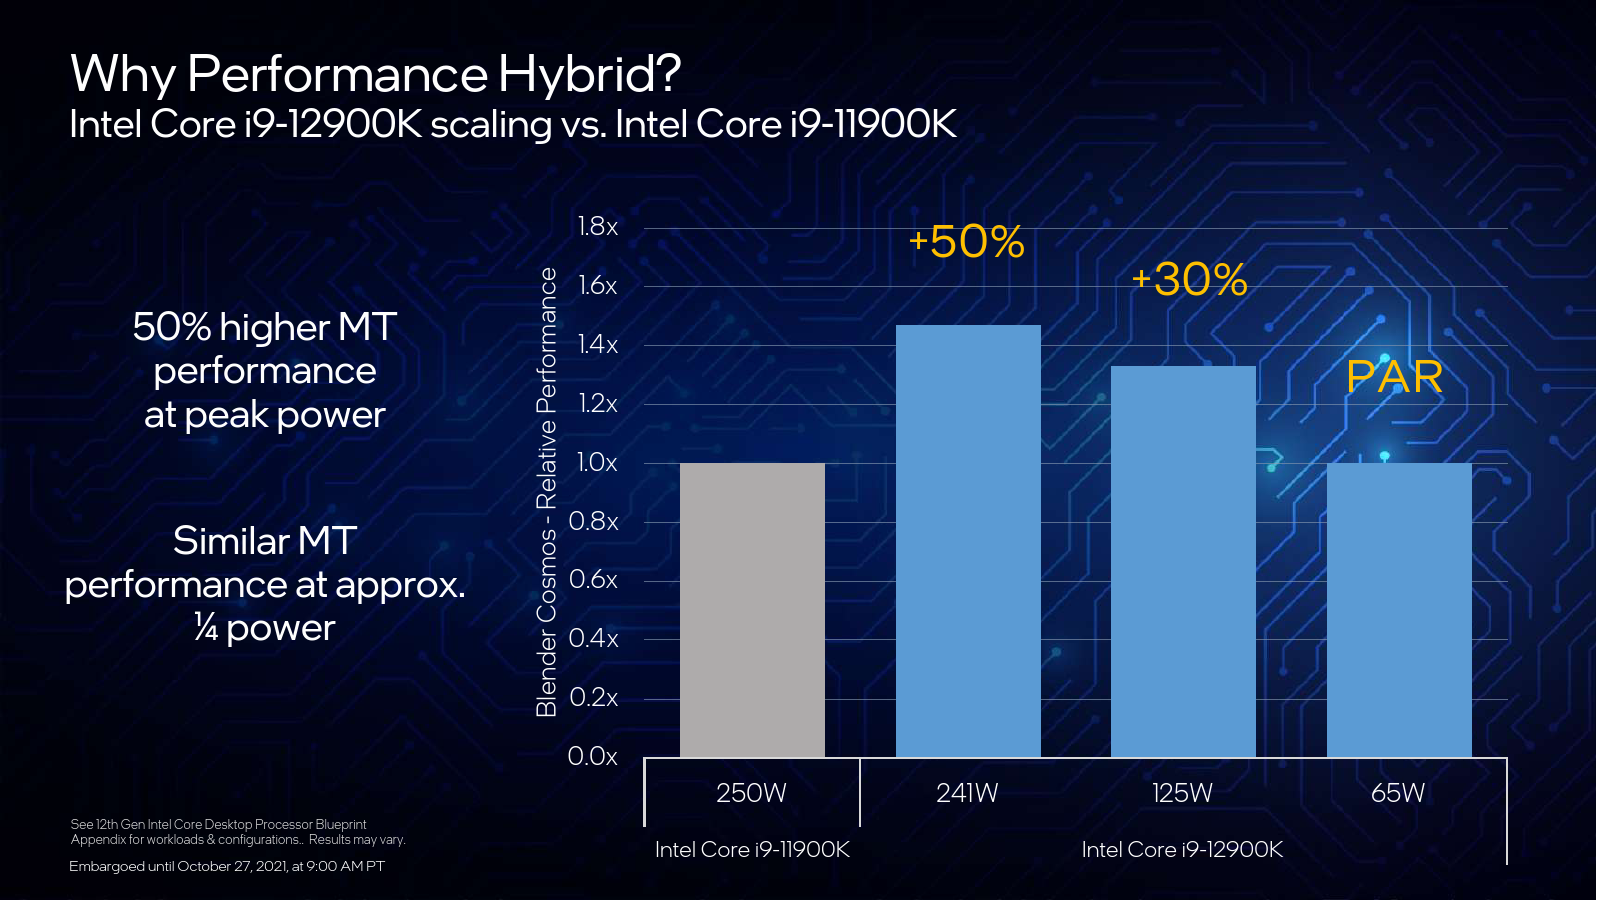
\includegraphics[width=0.7\textwidth]{12} %插入图片,[]中设置图片大小,{}中是图片文件名
\caption{Intel Core i9-12900K vs. Intel Core i9-11900K} %最终文档中希望显示的图片标题
\label{Fig.main2} %用于文内引用的标签
\end{figure}

\subsection{GPU}
RTX 3060 采用了GA106-300-A1核心,核心面积276mm2,CUDA数量为3584个,生产工艺是三星为NVIDIA定制的8nm工艺。RTX 3060 拥有1.32-1.78GHz 频率,配备了 12GB 192bit 位宽的 GDRR6 显存。这款显卡的官方功耗为 170W,配合 i9-10900K 需要 550W 电源。其浮点性能为 13 TFLOPS,张量性能可达 101 TFLOPS,光追性能则是 25 RT-TFLOPS。仅从规格上看,它的传统光栅化性能是 GeForce GTX 1060 的 2 倍,而光追性能则相比 GeForce GTX 1060 提升高达 10 倍。

\begin{table}[!htbp]
\centering
\begin{tabular}{|c|c|c|c|lllllllllllllllllllllllllllll}
\cline{1-4}
型号                                                          & RTX 3060                                                               & RTX 3070                                                               & RTX 2060 SUPER                                                                              &  &  &  &  &  &  &  &  &  &  &  &  &  &  &  &  &  &  &  &  &  &  &  &  &  &  &  &  &  \\ \cline{1-4}
核心代号                                                        & GA106-300                                                              & GA104-300                                                              & TU106-410                                                                                   &  &  &  &  &  &  &  &  &  &  &  &  &  &  &  &  &  &  &  &  &  &  &  &  &  &  &  &  &  \\ \cline{1-4}
核心面积(mm2)                                                   & 276                                                                    & 392.5                                                                  & 445                                                                                         &  &  &  &  &  &  &  &  &  &  &  &  &  &  &  &  &  &  &  &  &  &  &  &  &  &  &  &  &  \\ \cline{1-4}
制程 (nm)                                                     & 8                                                                      & 8                                                                      & 12                                                                                          &  &  &  &  &  &  &  &  &  &  &  &  &  &  &  &  &  &  &  &  &  &  &  &  &  &  &  &  &  \\ \cline{1-4}
GPCs                                                        & 3                                                                      & 6                                                                      & 3                                                                                           &  &  &  &  &  &  &  &  &  &  &  &  &  &  &  &  &  &  &  &  &  &  &  &  &  &  &  &  &  \\ \cline{1-4}
SMs/CUs                                                     & 28                                                                     & 46                                                                     & 34                                                                                          &  &  &  &  &  &  &  &  &  &  &  &  &  &  &  &  &  &  &  &  &  &  &  &  &  &  &  &  &  \\ \cline{1-4}
CUDA Cores/SP                                               & 3584                                                                   & 5888                                                                   & 2176                                                                                        &  &  &  &  &  &  &  &  &  &  &  &  &  &  &  &  &  &  &  &  &  &  &  &  &  &  &  &  &  \\ \cline{1-4}
Tensor Cores                                                & 112(第三代)                                                               & 184(第三代)                                                               & 272(第二代)                                                                                    &  &  &  &  &  &  &  &  &  &  &  &  &  &  &  &  &  &  &  &  &  &  &  &  &  &  &  &  &  \\ \cline{1-4}
RT Cores                                                    & 28(第二代)                                                                & 46(第二代)                                                                & 34(第一代)                                                                                     &  &  &  &  &  &  &  &  &  &  &  &  &  &  &  &  &  &  &  &  &  &  &  &  &  &  &  &  &  \\ \cline{1-4}
纹理单元                                                        & 112                                                                    & 184                                                                    & 136                                                                                         &  &  &  &  &  &  &  &  &  &  &  &  &  &  &  &  &  &  &  &  &  &  &  &  &  &  &  &  &  \\ \cline{1-4}
光栅单元                                                        & 48                                                                     & 96                                                                     & 64                                                                                          &  &  &  &  &  &  &  &  &  &  &  &  &  &  &  &  &  &  &  &  &  &  &  &  &  &  &  &  &  \\ \cline{1-4}
基础频率(MHz)                                                   & 1320                                                                   & 1500                                                                   & 1470                                                                                        &  &  &  &  &  &  &  &  &  &  &  &  &  &  &  &  &  &  &  &  &  &  &  &  &  &  &  &  &  \\ \cline{1-4}
Boost频率(MHz)                                                & 1882                                                                   & 1725                                                                   & 1650                                                                                        &  &  &  &  &  &  &  &  &  &  &  &  &  &  &  &  &  &  &  &  &  &  &  &  &  &  &  &  &  \\ \cline{1-4}
\begin{tabular}[c]{@{}l@{}}单精度浮点性能 (TFLOPS)\end{tabular} & 12.7                                                                   & 20.3                                                                   & 7/7.2                                                                                       &  &  &  &  &  &  &  &  &  &  &  &  &  &  &  &  &  &  &  &  &  &  &  &  &  &  &  &  &  \\ \cline{1-4}
显存                                                          & 12GB GDDR6                                                             & 8GB GDDR6                                                              & 8GB GDDR6                                                                                   &  &  &  &  &  &  &  &  &  &  &  &  &  &  &  &  &  &  &  &  &  &  &  &  &  &  &  &  &  \\ \cline{1-4}
\begin{tabular}[c]{@{}l@{}}显存数据速率 (Gbps)\end{tabular}     & 15                                                                     & 14                                                                     & 14                                                                                          &  &  &  &  &  &  &  &  &  &  &  &  &  &  &  &  &  &  &  &  &  &  &  &  &  &  &  &  &  \\ \cline{1-4}
显存位宽(bit)                                                   & 192                                                                    & 256                                                                    & 256                                                                                         &  &  &  &  &  &  &  &  &  &  &  &  &  &  &  &  &  &  &  &  &  &  &  &  &  &  &  &  &  \\ \cline{1-4}
显存带宽 (GB/s)                                                 & 360                                                                    & 448                                                                    & 448                                                                                         &  &  &  &  &  &  &  &  &  &  &  &  &  &  &  &  &  &  &  &  &  &  &  &  &  &  &  &  &  \\ \cline{1-4}
视频接口                                                        & \begin{tabular}[c]{@{}l@{}}HDMI 2.1×2\\ DisplayPort 1.4×3\end{tabular} & \begin{tabular}[c]{@{}l@{}}HDMI 2.1×1\\ DisplayPort 1.4×3\end{tabular} & \begin{tabular}[c]{@{}l@{}}HDMI 2.0b×1\\ DisplayPort 1.4×2\\ USB-C×1\\ DVI-D×1\end{tabular} &  &  &  &  &  &  &  &  &  &  &  &  &  &  &  &  &  &  &  &  &  &  &  &  &  &  &  &  &  \\ \cline{1-4}
TDP/TGP (W)                                                 & 170                                                                    & 220                                                                    & 175                                                                                         &  &  &  &  &  &  &  &  &  &  &  &  &  &  &  &  &  &  &  &  &  &  &  &  &  &  &  &  &  \\ \cline{1-4}
推荐电源(W)                                                     & 550                                                                    & 650                                                                    & 550                                                                                         &  &  &  &  &  &  &  &  &  &  &  &  &  &  &  &  &  &  &  &  &  &  &  &  &  &  &  &  &  \\ \cline{1-4}
供电接口                                                        & 8 Pin                                                                  & 12 Pin                                                                 & 8 Pin                                                                                       &  &  &  &  &  &  &  &  &  &  &  &  &  &  &  &  &  &  &  &  &  &  &  &  &  &  &  &  &  \\ \cline{1-4}
\end{tabular}
\caption{热门显卡规格参数对比}
\end{table}

\subsubsection{NVIDIA Ampere架构}
安培微架构(Ampere)是NVIDIA于2020年5月发布的一个GPU架构。用以取代图灵微架构(Turing microarchitecture)。命名为“安培”以向法国物理学家安德烈-马里·安培(André-Marie Ampère)致敬。Ampere架构拥有晶体管达540亿,是三星8nm级芯片。是世界上晶体管最多的芯片,直到后来被苹果M1 Max击败。

Ampere包含六项关键性的突破创新:
\begin{itemize}
  \item CUDA® 核心:与上一代相比,NVIDIA Ampere架构的CUDA核心可将单精度浮点 (FP32) 运算处理速度提升一倍,并将能效提升2倍。这显著改善了3D模型开发等图形工作流程的性能,另外还为计算机辅助工程 (CAE) 的桌面模拟等工作负载提供了强大算力。
  \item 第二代RT Cores:第二代RT Core的计算吞吐量是上一代的2倍,并能同时运行光线追踪和着色或降噪功能,从而大幅加快工作负载的运行速度,例如电影内容的逼真渲染和产品设计的虚拟原型创建。这项技术还可加速渲染具有光线追踪效果的动态模糊画面,从而更快获得视觉准确性更高的结果。
  \item 第三代Tensor Cores:新的Tensor Float 32 (TF32)精度提供的训练吞吐量达到上一代的5倍,而且无需更改代码即可加速AI和数据科学模型的训练。从硬件上支持结构化稀疏使推理吞吐量提升一倍。 Tensor Core还通过DLSS、AI降噪等功能将AI引入到图形处理中,并增强了特定应用程序的编辑功能。
  
  另外,为了提高Tensor Cores训练AI时的效率,NVIDIA新创了一种名为TF32的数据类型,它拥有FP32的范围和FP16的精度,对于调用Tensor Core的操作,它会自动启用TF32进行处理。而没有调用Tensor Cores的操作将仍然走FP32的数据路径,Tensor Cores会自动读取FP32数据,在内部减精度进行运算,在最终输出的时候会将数据还原成IEEE标准。
  \begin{figure}[H] %H为当前位置,!htb为忽略美学标准,htbp为浮动图形
\centering %图片居中
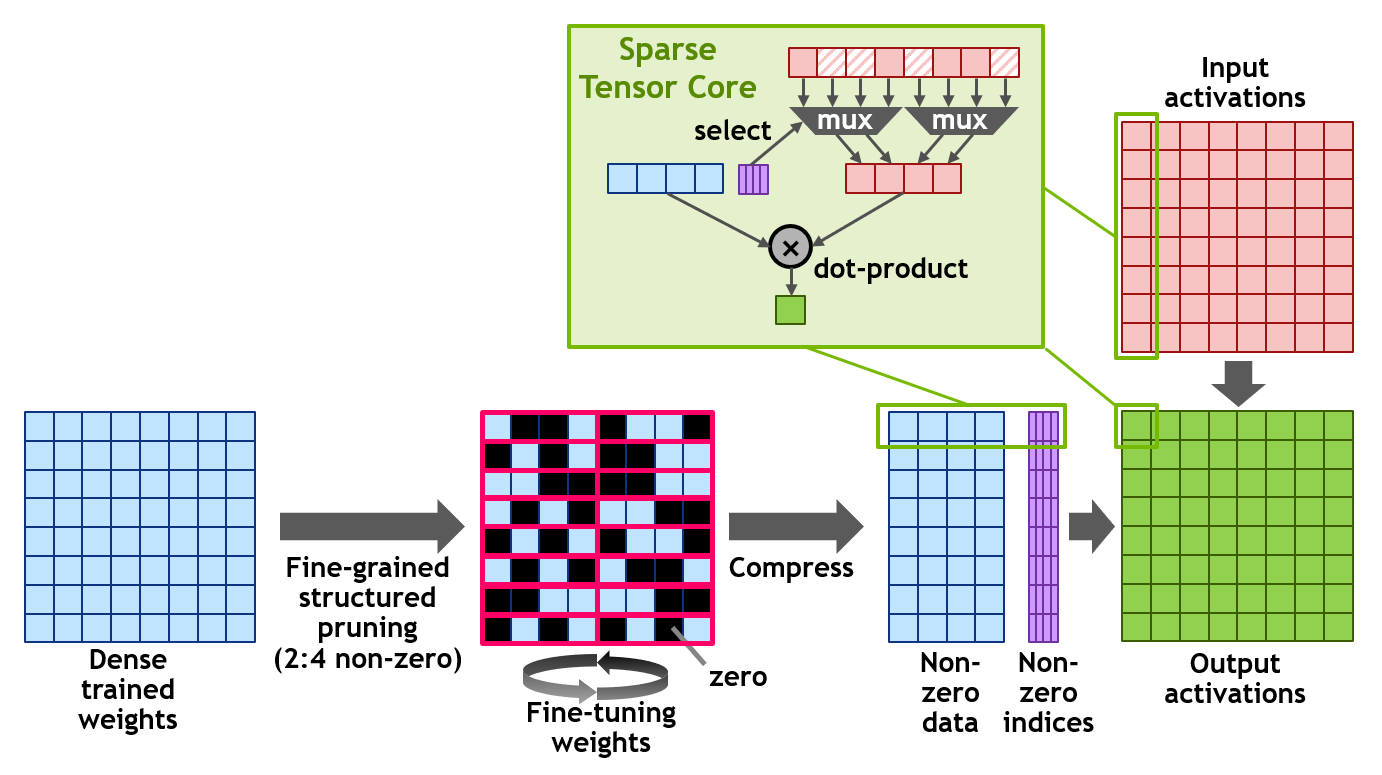
\includegraphics[width=0.7\textwidth]{tensor} %插入图片,[]中设置图片大小,{}中是图片文件名
\caption{计算流程演示} %最终文档中希望显示的图片标题
\label{Fig.main2} %用于文内引用的标签
\end{figure}

新版Tensor Cores还支持稀疏矩阵运算。稀疏矩阵指的是大部分元素为0的矩阵,对于这种矩阵,NVIDIA使用了自己开发出来的稀疏计算方式,它支持2:4的结构化稀疏运算,需要参与计算的矩阵在每四个元素中有2个以上的0元素,它可以将Tensor Cores的计算吞吐量翻一倍。
  \item PCI Express 4.0:基于NVIDIA Ampere架构的GPU支持PCI Express 4.0,该规范提供的带宽是PCIe第3.0代的2倍。这提高了从CPU内存传输数据的速度,可更好地执行AI和数据科学等数据密集型任务。更快的PCIe性能还能加速GPU直接显存访问(DMA)传输,从而能让支持视频的设备通过GPUDirect®更快速地传输视频数据,以及利用GPUDirect Storage加快输入/输出(I/O)速度。
  \item 第三代NVLink:第三代NVIDIA NVLink®技术允许用户将2个GPU连接起来,以分享GPU性能和显存。借助高达112千兆字节/秒(GB/s)的双向带宽和高达96 GB的组合显存,专业人员可以应对大型的渲染、AI、虚拟现实和视觉计算工作负载。新的NVLink连接器还具有更低矮的外形,可在更多型号的机箱中实现NVLink功能。
\end{itemize}

在图形计算方面,考虑到目前复杂的图形计算任务,NVIDIA采用的是FP32+INT32混组核心的设计,能够带来每晶体管性能的显著提升。

\section{总结}
\begin{itemize}
	\item i7-11800H在同系列处理器中属于中高产品,无明显短板,单线程性能强,多线程相对于AMD的5800H略差。
	\item 12代酷睿处理器的表现对得起众多DIY玩家长久的期盼,混合架构的设计被引入到了PC领域并且有着非常优秀的表现,相信未来PC领域的处理器都将追随英特尔的脚步推出混合架构设计的处理器。从这一点来看英特尔无愧是PC领域的引领者,与此同时也让人期待英特尔的移动标压处理器。
	\item Ampere架构的更新并不是革命性的,而是延续了NVIDIA这几年在架构设计上的一贯思路,微观上在SM单元中延续分精度计算,并加强Tensor Cores这个对深度学习计算非常有用的单元,宏观上面增大GPU的规模,不仅将整个GPU包含的SM单元数量扩大到128组这个数字,更是把整片GPU上面的缓存系统都放大了,尤其是40MB的二级缓存,让人印象深刻。

\end{itemize}


\newpage
\section{参考文献}
\cite{CPU1}\cite{CPU2}\cite{CPU3}\cite{GPU1}\cite{GPU2}\cite{GPU3}\cite{GPU4}
\bibliographystyle{plain}
\bibliography{reference.bib}

\end{document}